\begin{figure}[t]
    \centering
    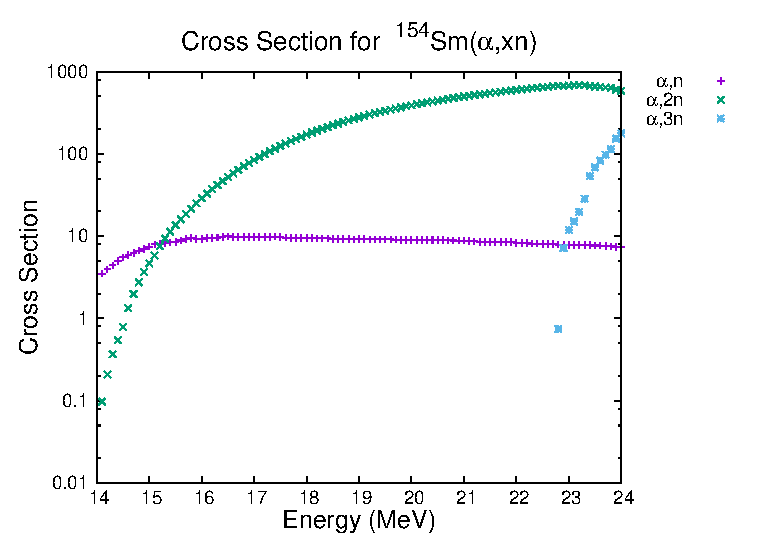
\includegraphics[scale=1]{Setup_Figs/alpha-n-comp.eps}
    \caption{Comparison between the cross sections of the $(\alpha,xn)$ reactions on $^{154}$Sm, calculated using Talys\citep{koning07:_talys}. The fewer neutrons being emitted, the lower the energy before the reaction occurs. Maximizing the cross section with respect to the neutron flux can be done by finding an energy where the desired reaction, $(\alpha,2n)$ can be maximized, while minimizing the $(\alpha,n)$ and $(\alpha,3n)$ reactions. Specifically, this means finding an energy before the $3n$ reaction has significant strength, while maximizing the $2n$ reaction, as the $n$ reaction is nearly the same across the energy regime of interest.}
    \label{fig:alpha-neutron}
\end{figure}